% Tento soubor nahraďte vlastním souborem s obsahem práce.
%=========================================================================
% Autoři: Michal Bidlo, Bohuslav Křena, Jaroslav Dytrych, Petr Veigend a Adam Herout 2019

% Pro kompilaci po částech (viz projekt.tex), nutno odkomentovat a upravit
%\documentclass[../projekt.tex]{subfiles}
%\begin{document}

\chapter{Úvod}
V~této práci je řešena implementace modelu systému hromadné obsluhy (SHO) se zaměřením na zábavní průmysl a jeho ekonomiku provozu. Naším konkrétním cílem je vytvoření a optimalizace ekonomického modelu Disneylandu, který, podle námi nalezených dat, má denní zisk 13,5 milionů dolarů. Na základě modelu a simulačních experimentů bude ukázáno, zda lze pomocí změny výdajů za reklamy přilákat více zákazníků a tím dosáhnout vyšší ziskovosti.

\section{Podílející se osoby a zdroje}
Na této práci se podíleli autoři: \\
\begin{tabular}{|c|c|}
\hline
Michal Blažek & xblaze38 \\
\hline
Kryštof Michálek & xmicha94 \\
\hline
\end{tabular} \\ \\
Zdroje:
\begin{itemize}
    \item Ekonomický stav Disneylandu: \cite{michael2024}
    \item Účinek reklamy na zákazníky: \cite{smith2024}
    \item Korelace počasí a návštěvnosti: \cite{joo2012}
\end{itemize}

\section{Prostředí experimentálního ověřování}
Pro zajištění validity modelu byly použity reálné údaje Disneylandu, které byly získány a poté ověřeny z~několika různých webových zdrojů. Experimentální ověřování validity modelu probíhalo v~prostředí simulačních nástrojů poskytnuté v~rámci výuky předmětu Modelování a simulace na FIT VUT v~Brně.

\chapter{Rozbor tématu a použitých metod/technologií}
V~této kapitole se zaměřujeme na souhrn dat pro modelování systému Disneylandu. Podle informací z~článku zveřejněného na webu Pixie Dust and Passports\cite{grace2023} má Disneyland přibližně 34 000 zaměstnanců. Zaměstnanci dostávají hodinovou mzdu v~od 15 do 30 dolarů, v~našem systému použito 15 dolarů, protože většina zaměstnanců se nachází na této spodní hranici. Otevírací doba parku je od 9:30 do 22:00, pracovní doba je tedy 12,5 hodiny.

V~článku Countdown to Magic\cite{michael2024} jsou provozní náklady Disneylandu přibližně 7 500 dolarů denně, denní náklady na ohňostroje 45 000 dolarů. Disney, dle nalezených informací, každoročně investuje do marketingu 1 milion dolarů, což je přibližně 2 740 dolarů denně. Celkový denní obrat Disneylandu je 13,5 milionu dolarů, z~toho 5,5 milionu dolarů pochází z~hotelu, který pro zjednodušení neuvažujeme. Celkové denní výdaje Disneylandu se pohybují kolem 3,25 milionu dolarů. Po odečtení zisku hotelu a po odečtení všech výdajů vychází průměrná denní útrata jednoho návštěvníka přibližně na 210 dolarů.

Průměrný denní počet návštěvníků Disneylandu je 25 000. Každý návštěvník zaplatí vstupné ve výši 83 dolarů, přičemž na jídlo vynaloží přibližně 25 dolarů a na suvenýry 102 dolarů. Pro usnadnění přikládáme také odkaz na dokument, ze kterého předchozí článek čerpal informace\cite{disney2022}.

Studie naznačuje, že reklama zlepší návštěvnost Disneylandu o~3,17 \cite{smith2024}. Pokud jde o~vliv počasí, podle článku špatné počasí včetně deště může snížit návštěvnost na polovinu\cite{joo2012}.

\section{Použité postupy pro vytvoření modelu} 
Pro vytvoření modelu bylo nejprve nutné sesbírat relevantní informace o~reálném subjektu, kterým v~našem případě je Disneyland. Tento krok zahrnoval získání údajů o~provozních nákladech, počtu zaměstnanců, návštěvnosti a dalších důležitých parametrech. Následně bylo nutné tyto údaje přizpůsobit a zjednodušit tak, aby vyhovovaly potřebám modelu hromadné obsluhy (SHO). V~tomto projektu byla použita Petriho síť, která umožňuje efektivní modelování. Posledním krokem bylo přeškálování získaných dat na náš zjednodušený model, což zahrnovalo převod reálných hodnot na hodnoty použitelné v~simulačním prostředí.

\newpage
\section{Původ použitých metod a technologií} 
Použité metody a technologie byly získány z~následujících zdrojů: \begin{itemize} \item \textbf{Metody:} Metodické postupy byly převzaty z~výuky předmětu Modelování a simulace na FIT VUT v~Brně. Získané znalosti tvorby Petriho sítí nám umožnily efektivně modelovat chování Disneylandu v~různých podmínkách. \item \textbf{Technologie:} \begin{itemize} \item \textbf{Jazyk C++ a jeho standardní knihovny:} Pro implementaci modelu jsme zvolili programovací jazyk C++. Kromě standardních knihoven jazyka C++ jsme využili také standardní knihovny STL (Standard Template Library). \item \textbf{Knihovna SIMLIB:} Knihovna SIMLIB\footnote{\url{https://www.fit.vut.cz/person/peringer/public/SIMLIB/}} byla použita jako hlavní nástroj pro simulaci. Byla stažena z~oficiálních stránek a použita ve své nejnovější dostupné verzi. Tento nástroj nám umožnil efektivně vytvářet, testovat a analyzovat simulace našeho modelu Disneylandu. \end{itemize} \end{itemize}

\chapter{Koncepce - modelářská témata} 
Konceptuální model se snaží co nejvěrněji přiblížit reálnému stavu, který je popsán v~kapitole 2. Při jeho tvorbě bylo nutné zjednodušit některé prvky tak, aby byly použitelné v~našem modelu. Tato zjednodušení zahrnují přeškálování údajů o~reálném Disneylandu, sloučení několika provozních a jiných nákladů a také sloučení několika zdrojů příjmů. Pracovali jsme s~pracovní dobou Disneylandu, která je od 9:30 do 22:00, park je tedy otevřený po dobu 12,5 hodin denně.

V~reálném světě návštěvnost Disneylandu kolísá v~průběhu dne, což jsme v~našem modelu neimplementovali, nezaměřujeme se na kapacitní vytíženost parku, ale na vliv reklamy na počet příchozích zákazníků a celkový zisk. Průměrný denní počet návštěvníků Disneylandu je 25 000. Z~tohoto počtu jsme vycházeli při vytváření modelu, který předpokládá rovnoměrné rozložení návštěvníků během celého dne.

\section{Způsob vyjádření konceptuálního modelu} 
Model se skládá ze dvou hlavních částí. První část slouží jako časovač pro určení otevírací doby parku. To je klíčové pro správné fungování druhé části, kterou je samotný zábavní park. Na začátku každého dne je určena pravděpodobnost, zda daný den bude pršet. Špatné počasí má zásadní vliv na počet návštěvníků a tím i celkový denní výnos parku.

Model dále zahrnuje turnikety, jednotlivé atrakce a stánky s~občerstvením. Časy strávené na jednotlivých místech byly nastaveny na základě testování systému tak, aby průměrná útrata návštěvníků ve stáncích odpovídala reálným údajům o~útratách za občerstvení a suvenýry.

\section{Formy konceptuálního modelu} Konceptuální model Disneylandu je vyjádřen prostřednictvím Petriho sítě. Podrobný popis modelu a jeho vizualizace je uveden v~příloze 1. Zjednodušený model vytvořený pomocí Petriho sítě poskytuje přehledný a srozumitelný způsob, jak simulovat a analyzovat chování Disneylandu.

\chapter{Architektura simulačního modelu/simulátoru} 
Tato kapitola popisuje architekturu simulačního modelu, jenž byl vytvořen na základě konceptuálního modelu.

\section{Mapování abstraktního modelu do simulačního} 
Simulační model byl navržen tak, aby odpovídal konceptuálnímu modelu. Mapování jednotlivých prvků vypadá následovně:

\begin{itemize} \item \textbf{Třídy a objekty:} Tyto prvky reprezentují jednotlivé procesy v~modelu. V~projektu jsou implementovány třídy \textit{otevreno}, která implementuje otevírací dobu a počítání výdajů a příjmů, dále třídu \textit{generator} vytvářející objekty další třídy a to \textit{navstevnik}, který má například metody \textit{turnikety},  \textit{toaleta}, \textit{stanky}... které definují jeho chování v~parku.
Dále pomocné třídy \textit{prijmyZeVstupu} a \textit{prijmyZeStanku}, které přičítají vlastní vydělané peníze k~celkovým příjmům. 
 \end{itemize}

\section{Přehled hlavních komponent modelu} 
Model obsahuje následující komponenty, které simulují reálné procesy v~Disneylandu:


\subsection{Třída otevreno} Tato třída implementuje otevírací dobu, uchovává hodnoty příjmů a výdajů a určuje se v~ní marketingová strategie pro daný den. Dále je zde  každý den s~určitou procentuální pravděpodobností generován příznak deště.

\subsection{Třída generator} Tato třída implementuje generování návštěvníků a simuluje tak čas příchodu jednotlivých návštěvníků během dne. Příznak deště pak tento čas modifikuje.

\subsection{Třída navstevnik} Tato třída implementuje jednotlivé návštěvníky parku. Obsahuje metody \textit{Behavior}, která popisuje jak se návštěvník chová od příchodu do parku až po projití turniketů, \textit{vDisneyLandu} určující procentuální výběr další akce, \textit{toaleta}, \textit{stanky}, ve kterých si pořídí jídlo či suvenýry, \textit{atrakce1, atrakce2 a atrakce3}, na kterých se zabaví nějaký daný čas, \textit{muzeOdejit}, určující procentuální šance odejití, a \textit{opousti}, kdy návštěvník opouští park.
\chapter{Podstata simulačních experimentů a jejich průběh}
Našim cílem bylo experimentováním zjistit, zda lze pomocí upravením výdajů na reklamy zvýšit návštěvnost Disneylandu a tím zvýšit jeho ziskovost.
\section{Postup experimentování}
Postup experimentování zahrnoval:
\begin{itemize}
    \item \textbf{cíl:} Navýšení zisku.
    \item \textbf{Plán experimentů:} Pomocí nastudované literatury upravit výdaje na reklamu a porovnávání výsledků našich experimentů s~očekávanými výsledky. 
\end{itemize}

\section{Dokumentace jednotlivých experimentů}
Experiment byl dokumentován následujícím způsobem:
\begin{itemize}
    \item \textbf{Vstupní podmínky:} Program běží a simuluje Disneyland na základě předem nastavených vstupních podmínek v~souboru \texttt{config.hpp}. V~základu se provádí 100 simulací pro každou desátou hodnotu marketingu, kde každá simulace představuje 3 roky provozu Disneylandu.
    \item \textbf{Výsledky:} Data, získaná ze simulací, se vypíší na standardní výstup a nebo případně do souboru. Tato data jsou následně zpracována a z~nich jsou vytvořeny grafy na obrázku \ref{grafy}.
    \item \textbf{Plán pro další experiment:} Z~experimentu je patrné, že zisk společnosti může za určitých podmínek překonat výdaje i v~případě nezapočítání příjmy z~hotelů, které společnost vlastní, tudíž není potřeba provádět další experimenty. Mezi další experimenty by mohlo například patřit zahrnutí slevy na vstupné a s~tím očekávané zvýšení zájmu návštěvníků.
\end{itemize}

\section{Závěry experimentů}
Bylo provedeno několik experimentů ohledně návštěvnosti a útratě jednotlivých návštěvníků za účelem přiblížení se reálným hodnotám návštěvnosti a ziskovosti společnosti. Další experimenty se týkají pokusu o~překonání výdajů společnosti pouze na základě zvýšení reklamy. Z~experimentů lze odvodit chování systému s~dostatečnou věrohodností.

V~grafech na obrázku \ref{grafy} se společnost aktuálně nachází na hodnotě marketingu 1, což naznačuje 1 milion dolarů ročně utracený na reklamy a jiné marketingové strategie. Z~grafu střední hodnoty příchodu návštěvníků závislé na velikosti marketingu lze vyčíst údaje o~zvýšení zájmu návštěvníků o~tento park v~různém počasí na základě velikosti marketingu společnosti. V~grafu příjmů a výdajů na základě hodnoty marketingu rostou výdaje konstantně, neboť každé zvýšení reklamy stojí společnost určitou hodnotu. Na grafu příjmů je vidět logaritmické zvýšení z~důvodu vyššího počtu návštěvníků, které v~daný moment dokonce překoná i celkové výdaje společnosti. Lze tedy říct, že společnost by měla investovat do marketingových strategií přibližně 400krát větší částku než nyní pro zajištění maximálního zisku v~poměru s~výdaji.

\begin{figure*}[h]
    \centering
    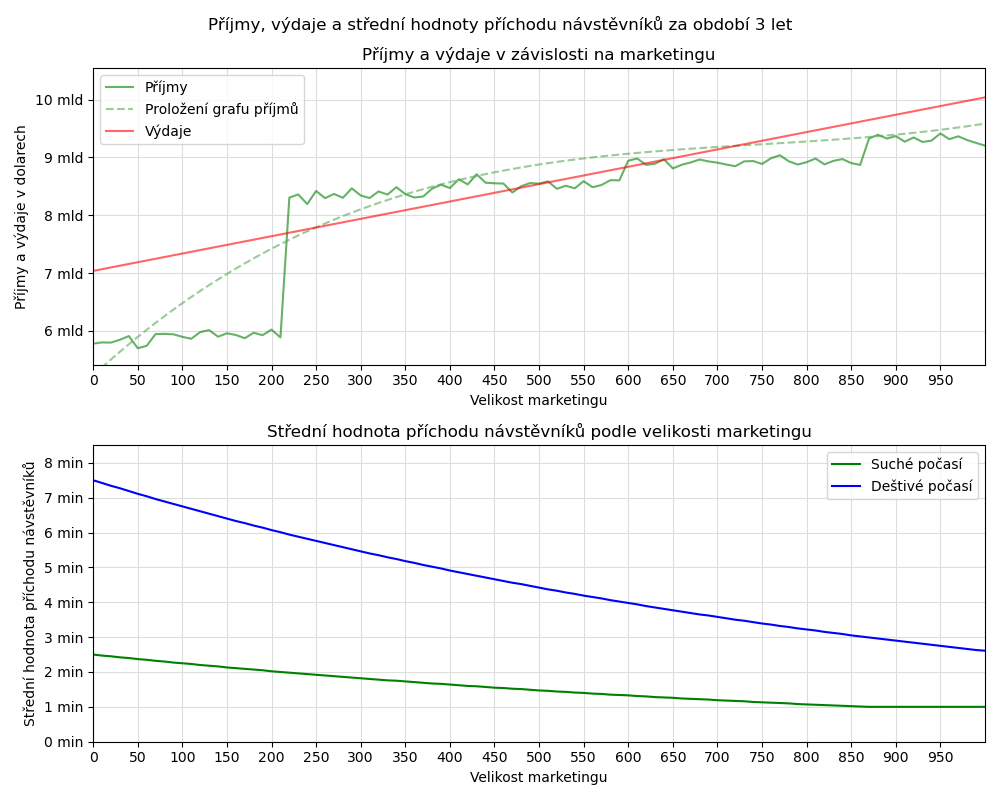
\includegraphics[width=1\textwidth]{obrazky-figures/graph.png}
    \caption{Velikost příjmů a výdajů na základě množství reklamy a střední hodnota příchodu návštěvníků podle zvýšené reklamy.}
    \label{grafy}
\end{figure*}
\chapter{Shrnutí simulačních experimentů a závěr}
Za pomocí systému hromadné obsluhy, přesněji pak Petriho sítě, jsme modelovali zjednodušený provoz zábavního parku Disneyland. Po získání, přeškálování a aplikování dat jsme pomocí pokusu ověřili validitu jak vlastního modelu, tak získaných dat. Po ověření validity jsme experimentováním zjistili, že zvýšením rozpočtu na reklamu je možné přilákat do zábavního parku více návštěvníků a tím zajistit jeho větší ziskovost.

%===============================================================================

% Pro kompilaci po částech (viz projekt.tex) nutno odkomentovat
%\end{document}
